\input{chapter-header.tex}
% ===========================================================================
\chapter{The \Vtt Prototype}
\minitoc
\chaplabel{prototype}
% ===========================================================================
\introduction
% ===========================================================================

To validate our model, we implemented our \Vtt prototype on the Pharo platform~(Section \ref{sec:pharo_execution_model}). Our solution virtualizes Pharo application runtimes and provides, as already described, the ability to manipulate their object graph and control their execution. Our implementation includes a language side library containing the object space and language hypervisor related classes. Our main modification to Pharo is an extension to its stack-based \VM. This \VM is a version of the Pharo \VM without its Just In Time~(JIT) compiler. We made the choice of the JIT-less VM to simplify the development efforts of our prototype. Our extension allows the co-existence of several application runtimes on the same \VM and the modification of the \VM setup interface.

We implemented object spaces by exposing Pharo's \emph{special objects array}. This array provides an object space with support to modify the \VM setup interface~(Section \ref{sec:setup_interface}) and to replace the \VM interpreter state to execute several co-existent application runtimes on top of the same \VM~(Section \ref{sec:context_switch}). \Vtt mirror's do not require particular changes in the Pharo \VM~(Section \ref{sec:implementation_mirrors}). We base our mirror implementation in two existing \VM primitive operations that allows us to execute a primitive on an arbitrary object by changing the primitive's receiver. Additionally, the already existing reifications of objects such as \ct{CompiledMethod}, \ct{Process}~(threads) and \ct{Context}~(stack frames or activation records), allow us to manage such runtime elements using the same mirror mechanism and avoid the development of specific ad-hoc solutions.

\Vtt presents a memory layout where the objects of both the virtualized runtime and the hypervisor co-exist in the same heap~(Section \ref{sec:memory}). This means on one side that there is no need for implementing special support on \emph{cross-runtime references} for mirrors. On the other side, we can reuse the existing memory management in the virtual machine almost transparently.

This chapter finishes, with means of completion, by presenting the non-implemented aspects of our solution: JIT compilation, shared state enforced by \VM implementation and correct management of external resources such as files or sockets~(Section \ref{sec:not_yet_implemented}).

\section{Pharo Execution Model in a Nutshell}\label{sec:pharo_execution_model}

To understand the constraints and limitations of our solution, we start this chapter by presenting the execution model imposed by the Pharo \VM. The Pharo \VM features a bytecode-based stack interpreter with a generational garbage collector and a JIT compiler. For the interested reader, several publications describe its details and how it evolved during time~\cite{Gold83a,Inga97a,Mira11a}. On the execution model side, this \VM imposes us the following contract:

\begin{description}

\item[Object Format.] All objects in the 32 bit version of the Pharo \VM have a header and a list of fields. The object header is one, two or three words long and describes amongst others how large is the field list of the object, if those fields contain weak or strong pointers, and which is the class of the object. The \VM also assumes the format of other special objects such as classes, method dictionaries and methods. Each class must have three mandatory fields: the superclass, its method dictionary and an integer describing the class format. Method dictionaries are hash tables that base their hash function on the identity of key objects. Methods are objects that contain a list of bytes with the bytecodes of the method and a list of the literal objects of that method encoded in the bytes.

\item[Object Model.] The Pharo \VM enforces, in its lowest level, a class-based object oriented model with single inheritance. Each object has a reference to its class~(that appears inside its header). Each class has only one superclass~(or \ct{nil} denoting the end of the hierarchy) and one method dictionary. The \VM during its execution does not enforce the existence of metaclasses nor a particular class hierarchy. Instead, meta-classes are built on top of this much simpler model. Indeed, this simple model allows one to implement other language extensions such as Traits~\cite{Scha03a} or mirrors as in Metatalk\cite{Papo11a}.

\item[Bytecode set.] The Pharo \VM constrains methods to a limited amount of predefined bytecode sets. These bytecode sets are based on the \VM's stack based interpreter. This means that every language that is meant to run on top of this \VM must be compiled to any of these bytecode sets, independently of its original syntax and semantics. 

\end{description}

\section{The Special Objects Array as \VM-Setup Interface}\label{sec:setup_interface}

Pharo \VM holds the state of the \VM-setup interface inside a \emph{special objects array} object. Pharo's special objects array contains 56 entries whose indexes are well known by the \VM for their access at runtime. To implement our \VM-setup interface, we expose, access and modify this special object array. Following, we detail the special objects array entries that we expose for our solution.

\begin{description}
\item[Special Instances.] Special instances such as \ct{nil}, \ct{true} and \ct{false} are directly pushed by the \VM interpreter at runtime instead of residing in a method literal list. A flyweight \ct{Character} table references the first 256 character objects to ensure their identity and save memory.

\item[System Dictionary.] The system dictionary references all installed classes in the system. An object space uses this entry to query the installed classes and to install new ones. The \VM does not make any special use of this object as it is managed directly from the language.

\item[Process Scheduler.] The process scheduler references all existing processes/threads in the runtime. We can install and remove process from the process scheduler. The \VM uses this same process scheduler to manage the runtime's execution.

\item[Symbol Table.] The symbol table gathers the set of \emph{unique} strings in the system. Symbols are mainly used to denote method signatures and ensure reference equality during the method lookup. An object space uses the symbol table to map symbols between runtimes and so it ensures no duplicate symbols are created. The \VM does not make any special use of this object as it is managed directly at the language level.

\item[Literal Classes.] Literal classes are the classes of literal objects. Literal objects are those objects whose values are known at parse time. The most known examples of literal objects are strings, numbers or literal arrays. These literal objects are then encoded inside the method where they are embedded. For example, numbers are usually included inside the method's literal list. Other literal objects such as block closures cannot however be created at compile time because they require to know runtime information, such as the stack context where they were created. Those objects are instead encoded in the method's bytecode. Then, the \VM creates at runtime a \ct{BlockClosure} instance when it finds the corresponding bytecodes. Generally speaking, on one side, the \VM uses the classes available in this list to directly instantiate objects of these types or perform safety checks at runtime~(which cannot be performed at compile time because of reflection or the dynamically-typed nature of the language). On the other side, an object space uses these well-known classes to perform transformations between objects in one runtime to another \eg translate a string from the hypervisor runtime to a string in the virtualized runtime.

\item[Special Selectors.] The special selectors denote those messages that the \VM will send to the image under special situations. This is the case of the \ct{doesNotUnderstand} selector that is sent to the receiver object when the method lookup fails finding a method under a message-send. Other selectors in this category are for example (a) \ct{cannotInterpret} which is sent when a class is involved in the method lookup with no method dictionary, (d) \ct{run:with:in:} when the method lookup finds in the method dictionary an object that is not a method, (c) \ct{mustBeBoolean} which is sent when a branch operation founds a non-boolean object.

\end{description}



%Particularly, the special objects array contains a process scheduler object and its corresponding process objects, implementing green threads. Pharo virtual machine has a single threaded nature and uses green threads to organize its execution.

\section{Cycle Execution and Context Switch} \label{sec:context_switch}

The Pharo \VM has single threaded execution \ie only one operating system thread is used to execute Pharo code. Process scheduling is handled internally by the virtual machine. Processes scheduled using this approach are also called \emph{green threads}. Green threads provide process scheduling without native operative system support while limiting the proper usage of modern multicore CPUs. By using green threads only one process, the \emph{active process}, is executed at each instant in time. If there are any waiting processes with a greater priority, the active process gets preempted \ie it is suspended and the process with the highest priority becomes the new active process.

In \Vtt, we modified part of the green thread mechanism to allow the scheduling of different application runtimes. We call \emph{context switch} the mechanism that changes from one application runtime to another. A virtualized application runtime runs for a window of time after which it gets preempted if another runtime with higher priority~(the language hypervisor runtime) is waiting. Internally, the \VM has a single bytecode interpreter shared amongst the different running runtimes. To perform the context switch, we exchange the special objects array of the \VM interpreter by the one from the application runtime to resume, and then resume the \VM execution~(cf. Figure \ref{fig:context_switch}). This solution keeps the single threaded nature of the \VM: the application runtime under execution is the \emph{active} application runtime while the others are considered as \emph{suspended} ones. This implementation has the benefit of avoiding concurrency problems between the different application runtimes, allowing us to focus on the runtime modification features.

\begin{figure}[ht]
\begin{center}
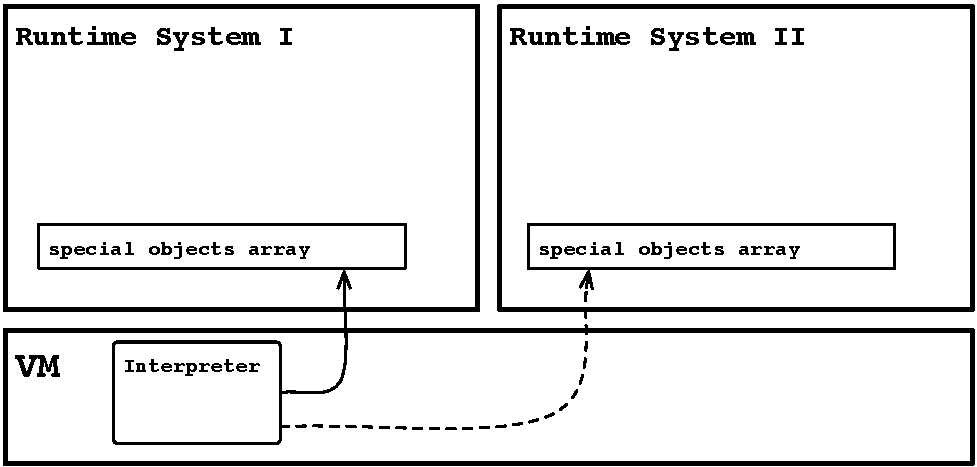
\includegraphics[width=.8\linewidth]{object_space_context_switch}
\caption{\textbf{Context Switch Internals.}To perform a context switch, we change the special objects array of the \VM's interpreter.\label{fig:context_switch}}
\end{center}
\end{figure}

Finally, the window time control was implemented hooking into the existing process preemption mechanism in the \VM. A separate \VM thread independent of the application runtimes, namely the \emph{heartbeat}, is awaken with a frequency of 5Hz~(\ie every 200 milliseconds) and activates a flag that indicates a preemption may occur. The chosen frequency is indeed important as it determines the precision of the clock measurements and how often the \VM checks for events such as delays or semaphores being signalled. If the frequency is unstable or low the clock resolution will be poor, delays will fire erratically and input from outside the \VM won't be responded to promptly.

When the \VM interpreter arrives to one of the safe suspension points (\ie a point where suspending the current execution will not leave the current process in a incoherent state) the code interpreter preempts the active process if the heartbeat signalled so~\cite{Deut84a}. Our safe suspension points correspond to the Cog \VM suspension points: back jump and message-send bytecodes~\cite{Mira11a}. This suspension points are designed on one side to minimize the execution overhead and on the other side to not suspend a process in between of a bytecode combination that could be unknown by the debugger. The suspension point before a message-send corresponds with the \VM's stack-overflow check and the one in backjumps allows preemption to happen in the case of long run (possible infinite) cycles. In \Vtt we modified the preemption code to activate another application runtime if available.

\section{\Vtt Mirror Implementation}\label{sec:implementation_mirrors}

We implement mirrors in \Vtt through the direct manipulation of the objects inside an object space. A \Vtt mirror includes a direct reference to its \emph{target}, an object inside an object space. The isolation between the hypervisor and the object space is handled by mirrors. The only object with grants to reference an object from other runtime is a mirror. To accomplish this, the operations on mirrors may yield either another mirror or objects that belong to the hypervisor runtime~(marshaled from their representation inside the object space).

\begin{figure}[htb]
\begin{center}
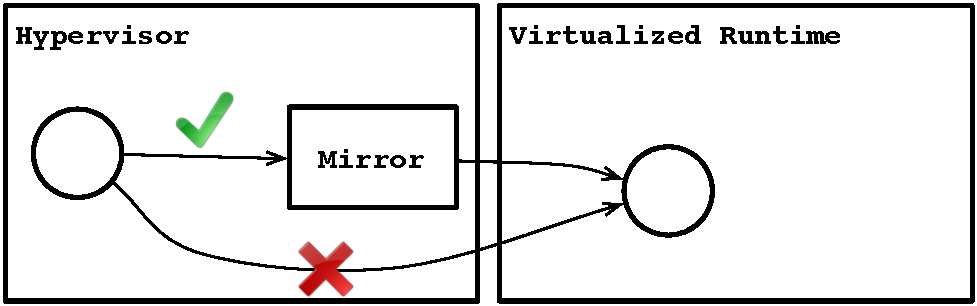
\includegraphics[width=.8\linewidth]{object_space_mirror_reference}
\caption{\textbf{Mirrors .}To perform a context switch, we change the special objects array of the \VM's interpreter.\label{fig:mirror_reference}}
\end{center}
\end{figure}

Mirrors manipulate their targets through \VM primitives. A primitive in Pharo is a function executed at the \VM level. The \VM assigns to each primitive an id, generally an integer index. To call a primitive at the language level we must add a method describing that it calls a primitive with a given id. Then, we have to send the corresponding message to the object subject of the primitive. The following code snippet shows an example where the size of an array is calculated by invoking a primitive. Primitive \textbf{62} is the primitive that returns the amount of variable fields of an object \eg the amount of fields of an array. For it, we make a method \ct{size} available in the \ct{Array} class implemented as a primitive invocation with a \emph{pragma} or annotation \ie the message-like expression between angle brackets~(<>). When sending the message \ct{size} to an array object, this method is looked up and found in this object class hierarchy, and the VM activates the primitive on the receiver object.

\begin{code}
Array >> size
    <primitive: 62>

"Then we can execute"
{1 . 2 . 3} size.
\end{code}

We want, however, to avoid cross-runtime message-sends. We then bypass the message-send with the combination of two existing primitives:
\begin{description}

\item[receiver:withArguments:executeMethod:] This primitive executes a \emph{given method} on an object. Given a method, it is possible to execute it on an object, avoiding method lookup in the object. In current Pharo \VM, this primitive is available in the \ct{CompiledMethod} class with the number 188. This method receives as arguments the object on which the primitive will be executed, an array of arguments, and the methods to execute.

\item[tryPrimitive:withArgs:] This primitive executes a \emph{primitive} on an object. It is possible to send a message to an object, so a primitive is executed on the receiver. This primitive is implemented in Pharo's \ct{ProtoObject} class as \textbf{\ct{tryPrimitive:withArgs:}} with number 118 and receives as argument the number of the primitive and an array or arguments.
\end{description}

Our mirrors use then a combination of these primitives to execute an arbitrary primitive while avoiding the method lookup. We use \ct{receiver:withArguments:executeMethod:} to execute the primitive method \ct{tryPrimitive:withArgs:} on the object from the virtualized runtime. The first avoids performing a message-send to the object inside the virtualized runtime. The second provides the ability to execute any arbitrary primitive. The following code snippet illustrate the how we implemented the \ct{size} primitive using mirrors.

\begin{code}
Mirror >> size
    ^ self executePrimitive: 62

Mirror >> executePrimitive: aPrimitiveNumber 
    ^ self executePrimitive: aPrimitiveNumber withArguments: #()
    
Mirror >> executePrimitive: aPrimitiveNumber withArguments: anArrayOfArguments
    "target is a reference to an object inside an object space"
    ^ CompiledMethod
           receiver: target
           withArguments: { aPrimitiveNumber . anArrayOfArguments }
           executeMethod: (ProtoObject >> #tryPrimitive:withArgs:)
\end{code}

Using this mechanism, \Vtt prototype implements one mirror per type of object supported by the Pharo \VM. Notice that as some runtime elements such as methods, activation records or even processes are reified as objects in Pharo, we can manipulate them through mirrors without developing new support for them in the \VM:

\begin{description}
\item[Object mirrors.] Mirrors for objects containing just object references such as an \ct{Array} or a \ct{Person}.
\item[Word mirrors.] Mirrors for objects containing only non-reference word size fields such as a \ct{Float} or a \ct{WordArray} object.
\item[Byte mirrors.] Mirrors for objects containing non-reference byte size fields such as a \ct{ByteArray} or a \ct{ByteString}. 
\item[Class mirror.] Mirrors for class like objects. They control the manipulation of classes and enforce the format of a class in the Pharo \VM which should necessary have as its first three instance variables the superclass of the class, its format and method dictionary.
\item[Method dictionary mirror.] Mirrors for method dictionaries enforcing the \VM invariants for method installation \ie using the identity as a hash for the key object for doing the lookup in the method dictionary.
\item[Method mirror.] Mirrors for method objects. Method objects in the Pharo \VM are objects with a mixed format. They contain object references to their literals, and byte fields with their bytecode.
\item[Context mirror.] Mirror for context objects. A context object is reified lazily by the Pharo \VM and contains a variable amount of fields denoting the local variables of a scope.
\item[Process mirror.] Mirror for process objects. Process objects are used to manage the execution of a Pharo runtime. They can be resumed, suspended or finalized.
\end{description}


%Using Oz, we can also create and install new processes inside an \objectspace given a code expression. The creation of a process requires the creation of a compiled method with the code~(bytecode) corresponding to the desired expression and a method context. The compiled method with the code to run is obtained by compiling the expression in the host and creating an \objectspace compiled method. The \objectspace compiled method is then provided with the compiled bytecode and its corresponding literals.

\section{\Vtt Virtual Interpreter} \label{sec:memory}

We implemented a virtual code interpreter for \Vtt by extending the existing Pharo's AST interpreter. Pharo's AST is able to parse Pharo code into AST, and execute it into the application runtime it belongs to by using reflection. We extended this AST interpreter with the purpose of executing the given AST inside an object space instead of inside the current application runtime. Our extensions include the following main points:

\begin{description}
\item[Name Resolution.] Names inside the source code representing \eg classes or globals must be resolved to the corresponding elements inside an object space. For this, we provide an alternative source of bindings to the AST semantic analysis process.

\item[Instance Variable Access.] Accessing or writing an object's instance variable is mapped by the code interpreter to a field access or write in the mirror representing the receiver object.

\begin{code}
VirtualCodeInterpreter >> readInstanceVariableNumber: index
    ^ self receiver instanceVariableAtIndex: index
    
VirtualCodeInterpreter >> writeInstanceVariableNumber: index with: aMirror
    ^ self receiver instanceVariableAtIndex: index put: aMirror
\end{code}

\item[Method Lookup.] On a message-send, the virtual code interpreter performs the method lookup by inspecting the class hierarchy of the receiver object. The receiver object state is exposed to the interpreter by a mirror. Following, we illustrate this with a simplified method lookup:

\begin{code}
VirtualCodeInterpreter >> lookupSelector: selector
    | classToLookup |
    "classToLookup is a class mirror"
    classToLookup := self receiver getClass.
    [ classToLookup isNotNil ] whileTrue: [
        (self class: classToLookup hasSelector: selector)
        	    ifTrue: [ ^ classToLookup ].
	classToLookup := classToLookup superclass.
    ]
\end{code}

\item[Primitive Execution.] In the leaves of the execution, message-sends invoke the language primitives. These language primitives are executed through the object space interface.

\begin{code}
VirtualCodeInterpreter >> invokePrimitiveMethod: aMethod
    ^ self receiver
         executePrimitive: aMethod primitive
         withArguments: self arguments
\end{code}

\end{description}

Being a first-class entity, we can specialize the code interpreter to instrument code execution in order to override normal behavior or trace the execution. We can for example trace all instance variable writes by overwriting one of the methods above.

\begin{code}
TracingCodeInterpreter >> writeInstanceVariableNumber: index with: aMirror
    | result |
    result := super writeInstanceVariableNumber: index with: aMirror.
    !\emph{self logWriteIn: self receiver atIndex: index with: aMirror.}!
    ^ result
\end{code}

\section{\Vtt Memory Layout} \label{sec:memory}

In \Vtt, all objects belonging to the different application runtimes share a unique object heap. Objects are mixed in this heap and objects from the same application runtime are not necessarily contiguous, as shown in Figure \ref{fig:heap}. However, Although they are mixed, they are logically separated as they belong to different object graphs. Pharo being a safe-language~\cite{Hawb98a,Hawb02a} prevents us to forge references~(\ie creating references from numbers using pointer arithmetic) and isolates the object graphs of each runtime system.

\begin{figure}[ht]
\begin{center}
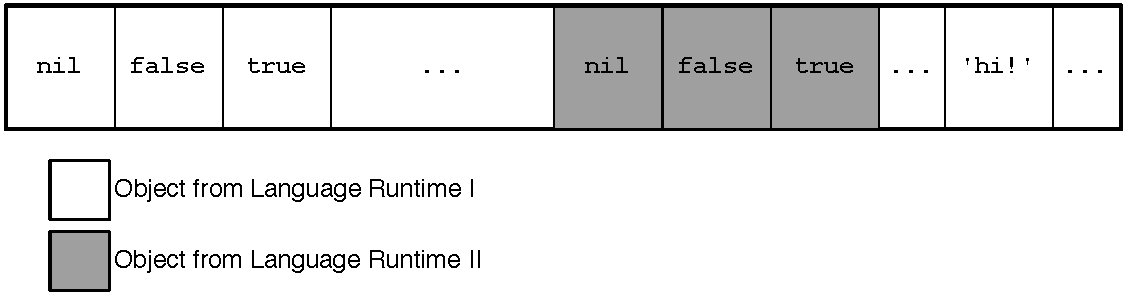
\includegraphics[width=.9\linewidth]{object_spaces_heap}
\caption{\textbf{A unique heap containing objects from different application runtimes.} Objects from the application runtime I and application runtime II are mixed in the heap. In this figure, after the \ct{nil}, \ct{true} and \ct{false} instances that belong to application runtime I, follow the corresponding ones of the application runtime II, which can in order be followed by objects of the former, like the string \textbf{`hi!'}. \label{fig:heap}}
\end{center}
\end{figure}

This decision is funded on minimizing the changes made to the virtual machine, to leverage the complexity in our prototype implementation. Our decision, while easing the development of our solution, has the following consequences:

\begin{description}
	\item[Reuse memory handling mechanisms.] We use the same existing memory infrastructure as when \Vtt is not used. Existing mechanisms for allocating objects or growing the object memory when a limit is reached can be reused transparently by our implementation. 
	\item[Simplify the object reference mechanism.] Cross-runtime references are normal object references. No extra support from the virtual machine was developed in this regard. Isolation is ensured at the language level through mirrors.
	\item[Shared garbage collection.] Since objects from the different runtimes are mixed in the object memory, and their boundaries are not clear from the memory point of view, the garbage collector~(GC) is shared between them. Every GC run must iterate over all their objects, increasing its time to run.
	\item[Limited to two co-existent application runtimes.] The current memory layout limits our prototype to two co-existent application runtimes due to the intervention of the CG and weak references. When the GC collects weak references, it replaces the reference to a reference to \ct{nil}. In the context of \Vtt, the GC should not replace weak reference to a unique \ct{nil} reference: it should replace it by a reference to the nil object from the correct application runtime. We can conclude that indeed, we need some kind of ownership mechanism \ie the GC may know to which application runtime an object belongs to correctly replace object references. In our prototype implementation we \emph{mark} ownership with only one available bit in the object header of objects. We look forward to replace this mechanism in the future by an alternative and more flexible implementation \eg separate memory regions per application runtime or extra object headers to represent ownership.
\end{description}

%This solution seems suitable  J-Kernel \cite{Hawb98a} and Luna \cite{Hawb02a} present a solution similar to ours regarding the memory usage. They are Java solution for isolating object graphs with security purposes. In them, each object graph is called a \emph{protection domain}. All protection domains loaded in a system, and their objects, share the same memory space. 

%The J-Kernel enforces the separation between domains by using the Java type system, the inability of the Java language to forge object references, and by providing capability objects\cite{Levy84a,Mill03a,Spoo00a} enabling remote messaging and controlling the communication. This same separation in Luna \cite{Hawb02a} is achieved by the modification of the type system and the addition in the virtual machine of the \emph{remote reference} concept. In our solution, the separation is given by the same inability to forge object references and the membrane objects that control the communication.

%\section{Creating an \objectspace} \label{sec:object_space_creation}
%
%An \objectspace can be created either from scratch or by loading an existing image. Loading an existing image was implemented as a virtual machine primitive, because the image snapshot is actually a memory snapshot and therefore, easier to handle at VM level. This primitive, implemented with the code shown in Figure~\ref{code:import_image}, reads the snapshot file, puts all objects into the object memory, updates the object references to make them coherent and finally returns the special objects array of the loaded image.
%
%\begin{figure}[htb]
%\begin{code}
%\textbf{primitiveLoadImage}
%    | headerlength bytesRead newImageStart rootOffset oldBaseAddress dataSize rootOop fileObject |
%    
%    "get the reference to the file object"
%    fileObject := self stackValue: 0.
%
%    "Where will we put the new objects"
%    newImageStart := objectMemory startOfFreeSpace.
%
%    "read image header"
%    self readLongFrom: fileObject.
%    headerlength := self readLongFrom: fileObject.
%    dataSize := self readLongFrom: fileObject.
%    oldBaseAddress := self readLongFrom: fileObject.
%    rootOffset :=
%          (self readLongFrom: fileObject) - oldBaseAddress.
%    
%    "seek into the file the start of the objects"
%    self seek: headerlength onFile: fileObject.
%    
%    "grow the heap in the ammount of the image size"
%    objectMemory growObjectMemory: dataSize.
%    
%    "read the file into the free part of the memory"
%    bytesRead := self
%                    fromFile: fileObject
%                    Read: dataSize
%                    Into: newImageStart.
%
%    "tell the vm the free space is now after the loaded objects"
%    objectMemory advanceFreeSpace: dataSize.
%         
%    "update the pointers of the loaded objects"
%    self
%          updatePointersForObjectsPreviouslyIn: oldBaseAddress
%          from: newImageStart
%          until: newImageStart + dataSize.
%    
%    "return the special objects array"
%    rootOop := newImageStart + rootOffset.
%    self pop: 2 thenPush: rootOop.
%\end{code}
%\caption{Implementation of primitive \textbf{\ct{primitiveLoadImage}} that loads an image snapshot into the object memory written in Slang
%\label{code:import_image}}
%\end{figure}
%
%On the other side, creating an \objectspace from scratch can be implemented as a bootstrap of the system, following the process defined in \cite{Poli12a}. The \objectspace provides the \textbf{\ct{createObjectWithFormat:}} method to create an object respecting the given format but with an anonymous class, so we can consider it as a "classless" object. This method is used in the first stage of the bootstrap process, when no classes are available in the \objectspace image yet, to create the \ct{nil} instance~(cf. Figure~\ref{code:bootstrap_nil}) and the first classes~(cf. Figure~\ref{code:bootstrap_classes}). Later, when the classes are available, those objects are set their corresponding ones by using the \textbf{\ct{setClass:}} message.

\section{Benchmarks}

We present in this section a series of benchmarks we applied to our implementation. The intent of these benchmarks is to provide an idea of the overhead that imply using our implementation of mirrors, process injection and the execution cycle. However, notice that the focus of this thesis is not on the performance of our technique for its extensive usage. Instead we focused on its flexibility for application runtime generation. We acknowledge that there is still pending work in the optimization of the techniques we used.

\subsection{Mirrors Micro-Benchmarks}

To evaluate the mirror usage overhead we measure six different aspects of our implementation: instance variable read and write, variable field read and write, object instantiation and primitive execution. We measured these aspects first in a normal program execution without reflection nor mirrors, second by using the standard reflection library provided by the language and finally by using mirrors. To have visible results, we used a problem size of 50000 between each measurement (\ie we actualle measured the time it took to execute 50000 times each benchmark).

\begin{table}[ht]
 	\centering
 	\begin{tabular}{lccc}%c|c|}
			\toprule
			\textbf{Benchmark}
			& \textbf{Normal}
 			& \textbf{Reflection}
			& \textbf{Mirrors}\\
		\midrule
		Instance Variable Read & 2.00ms +/-0.47 & 2.70ms +/-0.61 & 104.5ms +/-1.1 \\\midrule
		Instance Variable Write & 2.90ms +/-0.63 & 2.80ms +/-0.53 & 62.80ms +/-0.70 \\\midrule
		Variable Field Read &  \multicolumn{2}{c}{1.80ms +/-0.59}  & 105.20ms +/-0.45 \\\midrule
		Variable Field Write & \multicolumn{2}{c}{1.70ms +/-0.54}  & 63.00ms +/-0.97 \\\midrule
		Object Instantiation &  \multicolumn{2}{c}{3.20ms +/-0.93}  & 383.9ms +/-2.1 \\\midrule
		Primitive Execution & 1.60ms +/-0.67 & 3.50ms +/-0.78 & 89.40ms +/-0.82 \\\midrule
 	\end{tabular}
	\vspace*{0.2cm}
 	\caption{\textbf{Mirrors Micro Benchmarks.} Comparing the time to execute basic operations using the language as usual, using reflection and \Vtt mirrors.\label{tb:benchmarks}}
 \end{table}

As we can notice, this mirror implementation introduce a considerable overhead in execution when used. Table \ref{tb:benchmarks_percentages} shows the actual overhead by comparing the bechmark results. The overhead varies between 22 and 56 times the normal execution with the exception of object instantiation. We attribute this difference to the fact that object instantiation can trigger garbage collection every certain number of new objects created.

\begin{table}[ht]
 	\centering
 	\begin{tabular}{lcc}
			\toprule
			\textbf{Benchmark}
			& \textbf{Overhead}
 			& \textbf{Overhead}\\
		&\textbf{over}&\textbf{over}\\
		&\textbf{Normal Execution}&\textbf{Reflection}\\
		\midrule
		Instance Variable Read & 52x & 39x \\\midrule
		Instance Variable Write & 22x & 22x \\\midrule
		Variable Field Read &  \multicolumn{2}{c}{58x} \\\midrule
		Variable Field Write & \multicolumn{2}{c}{37x} \\\midrule
		Object Instantiation &  \multicolumn{2}{c}{116x} \\\midrule
		Primitive Execution & 56x & 26x \\\midrule
 	\end{tabular}
	\vspace*{0.2cm}
 	\caption{\textbf{Mirrors Overhead.} The actual overhead of using this mirror implementation over the normal language constructs.\label{tb:benchmarks_percentages}}
 \end{table}


\subsection{Process Injection Overhead}

To measure the overhead introduced by process injection over a normal message send, we present three different scenarios. The two first measure the injection of message sends that take a short time by only sending the \ct{yourself} message to an object. In the first case, the message is sent to a global object. In the second case the message is sent to a literal string, implying its marshalling to inside the object space during the injection of the process. The third scenario is the execution of a process that takes longer time~(the calculation of factorial of 5000). We compare each of these scenarios by executing them in out of the Espell infrastructure and by injecting them inside an object space. Benchmarks are run with a problem size of 5000 to have visible measurements \ie we run each benchmark 5000 times between measurements. Table \ref{tb:benchmarks_injection} shows our results.

\begin{table}[ht]

 	\centering
 	\begin{tabular}{lcc}%c|c|}
			\toprule
			\textbf{Benchmark}
 			& \textbf{Normal Execution}
			& \textbf{Process Injection}\\
		\midrule
		Single message-send (1) &0.40ms +/-0.48 & 38s +/-4 \\\midrule
		(1) with literal marshaling & 0.40ms +/-0.48 & 37s +/-0.1 \\\midrule
		Long message-send & 438s +/-18 & 521s +/-31\\\midrule
 	\end{tabular}
	\vspace*{0.2cm}
 	\caption{\textbf{Process Injection Benchmarks.} Measuring the overhead included in the execution by process injection.\label{tb:benchmarks_injection}}
 \end{table}

The results we obtained are measured in terms of a problem size of 5000, meaning that they are several orders of magnitude bigger than a single process injection. We then \emph{estimate} the overhead of process injection performing the following simple calculation~(cf. Table \ref{tb:benchmarks_injection_comparison}). Notice that we don't include in this calculation the confidence of the result. We can also see that the overhead is bigger in the case of smaller computations. This is explained by the cost of process injection, which depends on mirrors to create and install processes. However, the cost of process injection is payed only once per process injected when the process is created. We can see that in longer computations this cost is diluted.

\begin{equation*}
estimatedOverhead = \frac{processInjection}{normalExecution}
\end{equation*}

\begin{table}[ht]
 	\centering
 	\begin{tabular}{lc}
			\toprule
			\textbf{Benchmark}
 			& \textbf{Estimated Overhead}\\
		\midrule
		Single message-send (1) & 95070x \\\midrule
		(1) with literal marshaling & 91835x \\\midrule
		Long message-send & 1.18x  \\\midrule
 	\end{tabular}
	\vspace*{0.2cm}
 	\caption{\textbf{Process Injection Overhead.} Comparing the overhead included in the execution by process injection with the normal execution.\label{tb:benchmarks_injection_comparison}}
 \end{table}

\subsection{Execution Cycle Overhead}
With the objective of testing the execution cycle overhead, we executed a series of more complex benchmarks. We chose a subset of the computer language benchmarks game\footnote{\url{http://benchmarksgame.alioth.debian.org/}}. We executed each of these benchmarks ten times in three different setups. We first benchmarked the Vanilla JIT-less Pharo \VM without any of our changes, to make it a fair base of comparison with our JIT-less solution. Following, we benchmarked a non-virtualized solution running on our modified VM. Finally, we executed the same series of benchmarks using a Null hypervisor \ie an hypervisor that takes the execution control on each cycle and returns it to the object space without performing any particular action. Table \ref{tb:benchmarks} presents the results of our benchmarks, indicating the corresponding problem size of each benchmark.

%We executed each of these benchmarks in four different setups. Results are found in Table \ref{tb:benchmarks}. We first benchmarked the Vanilla JIT-less Pharo \VM without any of our changes, to make it a fair base of comparison. Afterwards, we benchmarked our solution in three different setups:

%\begin{description}
%\item[Null Hypervisor.] A hypervisor performing no action. This case is meant to measure the cycle overhead. 
%\item[File Checking Hypervisor.] A hypervisor that checks the existence of a File at each cycle. This case is meant to measure an action that does not include an interaction with the 
%\item[Stack Checking Hypervisor.] A hypervisor checking the execution stack of the virtualized runtime on each monitoring cycle. This benchmark forces in our prototype implementation a reification of the execution contexts~(stack frames) and the creation of several mirror objects.
%\end{description}

%\begin{landscape}
\begin{table}[ht]

 	\centering
 	\begin{tabular}{lccc}%c|c|}
			\toprule
			\textbf{Benchmark (problem size)}
 			& \textbf{Vanilla Pharo \VM}
			& \textbf{No Hypervisor}
			& \textbf{Null Hypervisor}\\
%			& \textbf{File Checking}
%			& \textbf{Stack Checking}\\
			
% 			\\& \textbf{}
%			& \textbf{}\\
%			& \textbf{Hypervisor}
%			& \textbf{Hypervisor}\\
		\midrule
		RegexDNA (10000) & 5711ms +/-22 & 5905ms +/-11 & 5878ms +/-18 \\\midrule% & 6142ms +/-11 & 6555ms +/-424 \\\midrule
		KNucleotide (1000)& 94.00ms +/-0.85 & 95.60ms +/-0.77 & 100.1ms +/-3.4\\\midrule% & 105.8ms +/-3.2 & 134.4ms +/-3.7 \\\midrule
		SpectralNorm (100) & 79.8ms +/-1.4 & 84.9ms +/-1.1 & 86.6ms +/-1.4\\\midrule% & 92.7ms +/-6.0 & 110.7ms +/-1.7 \\\midrule
		BinaryTrees (9) & 36.80ms +/-0.65 & 34.60ms +/-0.40 & 37.10ms +/-0.83 \\\midrule%& 35.30ms +/-0.66 & 65.20ms +/-0.93 \\\midrule
		Mandelbrot (200) & 422.3ms +/-1.4 & 468.8ms +/-2.9 & 488.0ms +/-6.5 \\\midrule%& 494.9ms +/-3.4 & 632ms +/-23 \\\midrule
		ReverseComplement (1000) & 5.40ms +/-0.48 & 6.00ms +/-0.71 & 6.80ms +/-0.24 \\\midrule%& 6.80ms +/-0.59 & 8.00ms +/-0.60 \\\midrule
		ThreadRing (1000) & 2.50ms +/-0.41 & 2.20ms +/-0.59 & 2.50ms +/-0.56\\\midrule% & 2.70ms +/-0.90 & 3.20ms +/-0.80 \\\midrule
		PiDigits (27) & 0.90ms +/-0.69 & 0.70ms +/-0.66 & 0.70ms +/-0.66 \\\midrule%& 0.70ms +/-0.66 & 0.90ms +/-0.69 \\\midrule
		Meteor (2098) & 2260.2ms +/-2.6 & 2373ms +/-12 & 2398.2ms +/-8.5 \\\midrule%& 2479ms +/-16 & 3677ms +/-267 \\\midrule
		NBody (1000) & 21.10ms +/-0.57 & 20.80ms +/-0.80 & 21.70ms +/-0.66 \\\midrule%& 22.6ms +/-1.4 & 37.7ms +/-1.5 \\\midrule
%		FannkuchRedux & 0.00ms +/-0.00 & 0.00ms +/-0.00 & 0.20ms +/-0.36 & 0.00ms +/-0.00 \\\midrule
		Fasta (1000) & 4.30ms +/-0.54 & 4.80ms +/-0.70 & 5.20ms +/-0.65 \\\bottomrule%& 5.70ms +/-0.61 & 9.30ms +/-0.39 \\\hline
 	\end{tabular}
	\vspace*{0.2cm}
 	\caption{\textbf{Execution Cycle Benchmarks.} Comparing the cycle overhead from a non virtualized Pharo VM to a virtualized one.\label{tb:benchmarks}}
 \end{table}
 
Given that each benchmark is executed as many times as big is its problem size between measurements, this measurements do not estimate the cost of one execution of it. Instead, we do a comparison of these times to \emph{estimate} the overhead of the execution cycle during each of these benchmarks~(Table \ref{tb:benchmarks_comparison}). Note that the biggest the time the benchmark takes, the more diluted the cost of process injection is. Notice also that we don't include in this estimation the confidence of the result, which in cases such as the PhDigits benchmark show that the results are spread. We do our estimations with the following calculation.

\begin{equation*}
estimatedOverheadOf(X) = \frac{measurementOn(X)}{normalExecution}
\end{equation*}

\begin{table}[ht]

 	\centering
 	\begin{tabular}{lccc}%c|c|}
			\toprule
			\textbf{Benchmark}
 			& \textbf{Espell VM Overhead}
			& \textbf{Hypervisor Overhead}\\
		\midrule
		RegexDNA & 1.03x & 1.03x \\\midrule
		KNucleotide & 1.02x & 1.06x \\\midrule
		SpectralNorm & 1.06x & 1.09x \\\midrule
		BinaryTrees & 0.94x & 1.01x  \\\midrule
		Mandelbrot & 1.11x & 1.16x \\\midrule
		ReverseComplement & 1.11x & 1.26x \\\midrule
		ThreadRing & 0.88x & 1x \\\midrule
		PiDigits & 0.77x & 0.77x \\\midrule
		Meteor & 1.05x & 1.06x \\\midrule
		NBody & 0.99x & 1.03x \\\midrule
		Fasta & 1.12x & 1.21x \\\bottomrule
 	\end{tabular}
	\vspace*{0.2cm}
 	\caption{\textbf{Execution Cycle Overhead.} Comparing the cycle overhead from a non virtualized Pharo VM to a virtualized one.\label{tb:benchmarks_comparison}}
\end{table}

\section{Non Implemented Aspects} \label{sec:not_yet_implemented}
 
For the sake of completion, we document in this subsection the aspects that have not been yet implemented in our prototype solution.

\subsection{JIT Compilation}

Just In Time~(JIT) compilation is available in the production distribution of the Pharo \VM. The existing JIT compiler doubles the performance of Pharo Stack \VM while adding yet another complex component in the \VM machinery. To reach such performance, it makes assumptions on the memory layout of the running application runtime. For example, it requires commonly accessed objects such as \ct{nil}, \ct{true} or \ct{false} to remain in the same memory position to optimize their access.

However, \Vtt introduces more than one application runtime in the same heap \eg more than one version of special objects such as \ct{nil} are present in the same heap. Moreover, these objects can be moved in memory on GC compaction. This breaks the \JIT assumptions. Thus, supporting JIT compilation in \Vtt would require a complete reengineering of the existing JIT compiler and possibly the \VM.

\subsection{Plugin and Native Libraries State}

Pharo \VM allows one to access resources from outside the application runtime through native libraries and \VM plugins. A \VM plugin is a native library that satisfies a particular interface to communicate with the \VM. Native libraries may keep their own state and may not be designed to be loaded several times in the same process. In particular, \VM plugins are often developed assuming the existence of only one application runtime so their state is global for the whole \VM.

The main \VM modifications we made in our prototype to support the basic execution of several application runtimes do not include modification on \VM plugins, nor it handles the case of loading multiple versions of the same native library from different runtimes. The usage of some of these elements in \Vtt may not be fully working.

\subsection{Finalization of External Resources}

Pharo \VM supports the concept of weak references. If an object is only referenced by a weak reference, this object will be garbage collected and this weak reference replaced by a reference to \ct{nil}. However, before garbage collecting the object, the \emph{finalization mechanism} will send the \ct{finalize} message to a finalizer object in charge of releasing any resources it may be holding. Finalization is useful to release resources external to the application runtime such as files or sockets. In Pharo, this finalization process is activated from the \VM but executed by the application runtime.

In \Vtt and because of the shared garbage collection, it may happen that a GC activated by one application runtime (the active application runtime) collects an object from another suspended application runtime. In such case, the \VM will activate only the finalization of the active application runtime. Then, the collected object from the suspended application runtime does not have the possibility to finalize its resources. This may cause external resource leaks, since they can be garbage collected but not properly finalized and released.
% ===========================================================================
\section{Conclusion and Summary}

This chapter explores the implementation aspect of our \Vtt prototype on the Pharo programming language. Our prototype includes a language-side library written for the Pharo and modifications in the Pharo \VM. We based our prototype in the \emph{Stack} Pharo \VM flavor. This \VM is the same as the production Pharo \VM except for the absence of a JIT compiler.

We implemented the \VM Setup interface by exposing Pharo's special object array, an array object referencing objects that the \VM access directly at runtime. This special array contains also the state of the code interpreter, as it references to the process scheduler of the language. Thus, by exchanging the special objects array of the \VM code interpreter we can make a context switch between different application runtimes.

Mirrors are implemented by the combination of existing \VM primitives and do not require new \VM support for their implementation. Our mirror hierarchy covers all kind of objects that the \VM support. Particularly, the already existing reification of execution-related elements such as processes and contexts allows us to implement their manipulation through mirrors and use the same mechanisms as for regular objects.

Regarding the chosen memory layout, in \Vtt all running application runtimes share the same object heap. This decision ease our prototype implementation as no special support for cross-runtime references is needed. However, this has an impact in the time consumed by the GC over a bigger heap.

The benchmarks we run let us make several conclusions. First, that there are improvements to make in our mirror implementation. Second, that our process injection implementations introduces an important overhead for the injection of smaller computations while it shows an acceptable overhead in the case of more longer computations. Finally, the game benchmark suite shows that the execution cycle control has an acceptable overhead that is for the majority of our benchmarks below the 10\%. We would also like to note that our implementation was biased towards its flexibility and no real effort was spent on optimizations, where there is still room for improvement. A fully engineered solution should improve on that an other points, specifically the JIT compiler, the state of native libraries and plugins, the shared GC and the problems in object finalization.

% =============================================================================
\input{chapter-footer.tex}